\chapter{Sincronizzazione dei Processi}

\section{Introduzione}
Più processi possono cooperare per compiere un determinato lavoro, e spesso \textbf{condividono dei dati}.

\begin{itemize}
    \item È fondamentale che l'accesso ai dati condivisi da parte dei vari processi non produca dati inconsistenti.
    \item I processi cooperanti devono quindi \textbf{sincronizzarsi} per accedere ai dati condivisi in modo ordinato.
    \item \textbf{Problema}: mentre un processo $P$ sta elaborando dati condivisi, il SO potrebbe toglierlo dalla CPU in qualsiasi momento. Altri processi non devono poter accedere ai dati condivisi finché $P$ non ha completato l'elaborazione.
\end{itemize}

\subsection{Esempio: Produttore-Consumatore con n eleemnti}
Usiamo una variabile \textbf{\textit{condivisa}} \textbf{counter} inizializzata a 0 che indica il numero di elementi nel buffer.

I due programmi sono corretti se considerati separatamente, ma possono non funzionare quando vengono eseguiti insieme.

\begin{itemize}
    \item Il problema risiede nell'uso della variabile condivisa \texttt{counter}.
    \item Che succede se il produttore esegue \texttt{counter++} mentre \textit{contemporaneamente} il consumatore esegue \texttt{counter--}?
    \item Se \texttt{counter} all'inizio vale 5, dopo \texttt{counter++} e \texttt{counter--} può valere 4, 5 o 6!
    \item N.B.: diciamo che possono non funzionare, e non che non funzionano, perché la condizione problematica potrebbe non verificarsi sempre.
\end{itemize}
Il problema si verifica perchè \texttt{counter++, counter--} non sono \textbf{operazioni atomiche}
Le operazioni sui dati condivisi possono portare a risultati imprevisti. Consideriamo le istruzioni per il \textbf{produttore} e il \textbf{consumatore} relative alla variabile condivisa \texttt{counter}:
\textbf{Produttore:}
\begin{verbatim}
load(registro1, counter);  % Carica il valore di counter in registro1
add(registro1, 1);         % Incrementa il valore nel registro di 1
store(registro1, counter);  % Salva il valore incrementato in counter
\end{verbatim}
\textbf{Consumatore:}
\begin{verbatim}
load(registro1, counter);  % Carica il valore di counter in registro1
sub(registro1, 1);         % Decrementa il valore nel registro di 1
store(registro1, counter);  % Salva il valore decrementato in counter
\end{verbatim}

Se il produttore e il consumatore accedono a \texttt{counter} in modo non sincronizzato, il valore finale di \texttt{counter} può risultare errato e instabile.


Quando i processi devono accedere e modificare dati condivisi, è fondamentale che si \textbf{sincronizzino} affinché ciascuno possa completare le proprie operazioni sui dati prima che un altro processo possa accedervi.

\begin{itemize}
    \item Questo approccio assicura l'integrità dei dati e previene condizioni di competizione.
    \item Da notare che il problema non si presenta se tutti i processi coinvolti nell'accesso a un insieme di dati condivisi devono solo \textbf{leggere} quei dati.
\end{itemize}


\section{Sezioni critiche}
Siano dati $n$ processi $P_1, \ldots, P_n$ che usano variabili condivise. 

 Ogni processo ha una porzione di codice, detta \textbf{sezione critica}, in cui manipola le variabili condivise (o anche solo un loro sottoinsieme).\\
 Quando un processo $P_i$ è dentro alla propria sezione critica, nessun altro processo $P_j$ può eseguire il codice della propria sezione critica, poiché userebbe le stesse variabili condivise (o anche solo un loro sottoinsieme).\\
 L'esecuzione delle sezioni critiche di $P_1, \ldots, P_n$ deve quindi essere \textbf{mutualmente esclusiva}.\\
Mentre un processo $P_i$ sta eseguendo codice nella propria sezione critica, potrebbe essere tolto dalla CPU dal sistema operativo a causa del normale avvicendamento tra processi. \\
 Fino a che $P_i$ non ha terminato di eseguire il codice della sua sezione critica, \textbf{nessun altro processo $P_j$ che deve manipolare le stesse variabili condivise potrà eseguire il codice della propria sezione critica}.\\
 \clm{}{}{
 È importante notare che $P_j$ può comunque eseguire del codice, quando entra in esecuzione, ma non il codice della propria sezione critica.
 }
\dfn{Sezione critica}{
Sezione critica: porzione di codice che deve essereeseguito senza intrecciarsi (nell’avvicendamento in CPU) col codice delle sezioni critiche di altri processi che usano le stesse variabili condivise
}

\subsection{Problema della Sezione Critica}
Per garantire l'accesso sicuro alle variabili condivise, è necessario stabilire un \textbf{protocollo di comportamento} per i processi. 

\begin{itemize}
    \item Un processo deve \textbf{“chiedere il permesso”} per entrare nella sezione critica, utilizzando una opportuna porzione di codice detta \textbf{entry section}.
    \item Un processo che esce dalla sua sezione critica deve \textbf{“segnalarlo”} agli altri processi, usando una opportuna porzione di codice detta \textbf{exit section}.
\end{itemize}

Un generico processo Pi contiene una sezine critica che avrà la seguente struttura
\begin{verbatim}
    altro codice
        entry section
        sezione critica
        exit section
    altro codice
\end{verbatim}
\bigskip
Siano dati $n$ processi $P_1, \ldots, P_n$ che usano delle variabili condivise. Una soluzione corretta al problema della sezione critica per $P_1, \ldots, P_n$ deve soddisfare i seguenti tre requisiti:

\begin{enumerate}
    \item \textbf{Mutua esclusione:} Se un processo $P_i$ è entrato nella propria sezione critica ma non ne è ancora uscito (attenzione, $P_i$ non è necessariamente il processo in esecuzione, cioè quello che sta usando la CPU), nessun altro processo $P_j$ può entrare nella propria sezione critica.
    \item \textbf{Progresso:} Se un processo lascia la propria sezione critica, deve permettere ad un altro processo $P_j$ di entrare nella propria (di $P_j$) sezione critica. Se la sezione critica è vuota e più processi vogliono entrare, uno tra questi deve essere scelto in un tempo finito (\textit{in altre parole, esiste un processo che entrerà in sezione critica in un tempo finito)}
    \begin{itemize}
        \item \clm{}{}{Qquesta condizione garantisce che l’insieme dei processi P1,… Pn (o anche solo un loro sottoinsieme) non finisca in una condizione di deadlock: tutti fermi in attesa di riuscire ad entrare nella loro sezione critica}
    \end{itemize}
    \item \textbf{Attesa limitata:} se un processo $P_i$ ha già eseguito la sua entry section (ossia ha già chiesto di entrare nella sua sezione critica), esiste un limite al numero di volte in cui altri processi possono entrare nelle loro sezioni critiche prima che tocchi a $P_i$ \textit{(in altre parole, \textbf{qualsiasi} processo deve riuscire ad entrare in sezione critica in un tempo finito)}
    \begin{itemize}
        \item \clm{}{}{Quest’ultima condizione assicura che il processo Pi non subisca una forma di \textbf{starvation}: non riesce a proseguire la sua computazione perché viene sempre sopravanzato da altri processi.}
    \end{itemize}
\end{enumerate}
Una qualsiasi soluzione corretta al problema della sezione critica deve permettere ai processi di portare avanti la loro computazione \textbf{indipendentemente} dalla velocità relativa a cui essi procedono (ossia da quanto frequentemente riescono ad usare la CPU), purchè questa sia maggiore di zero.\\
\textbf{Notate:} dire che la soluzione deve essere indipendente dalla velocità relativa a cui procedono i processi significa, più tecnicamente, che:
\begin{itemize}
    \item la soluzione non deve dipendere dal tipo di \textit{scheduling} della CPU adottato dal SO (ossia dall'ordine e dalla frequenza con cui i processi vengono eseguiti);
    \item purché, chiaramente, si usi un algoritmo di \textit{scheduling} ragionevole, come quelli che abbiamo visto.
\end{itemize}
Il problema della sezione critica è particolarmente delicato quando sono coinvolte strutture dati del sistema operativo.
\begin{itemize}
    \item Ad esempio, se due processi utente eseguono una \texttt{open} sullo stesso file, vi saranno due accessi concorrenti alla stessa struttura dati del SO: la tabella dei file aperti nel sistema.
    \item È importante che questa tabella (come tutte le strutture dati del SO) non venga lasciata in uno stato inconsistente a causa dell'accesso concorrente dei due processi.
\end{itemize}

\begin{figure}[h]
    \centering
    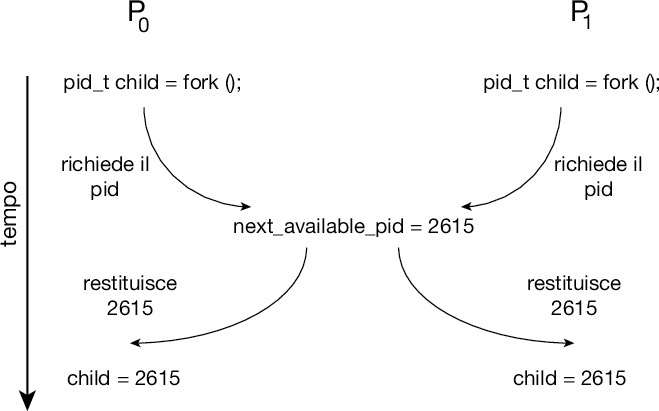
\includegraphics[width=0.5\linewidth]{images/kernel_sezioneCritica.png}
    \caption{il caso di due processi che eseguono “insieme” una fork: senza opportune precauzioni, potrebbero nascere nel sistema due nuovi processi con lo stesso PID!}
    \label{fig:kernel-criticSection}
\end{figure}
Il progettista del SO deve decidere come vanno gestite le sezioni critiche del sistema operativo, e le due scelte possibili sono di sviluppare un \textit{kernel} con o senza diritto di prelazione.
\begin{itemize}
    \item In un \textit{kernel} \textbf{con} \textbf{diritto di prelazione}, un processo in \textit{kernel mode} può essere interrotto da un altro processo (ad esempio, perché è scaduto il quanto di tempo).
    \item In un \textit{kernel} \textbf{senza diritto di prelazione}, un processo in \textit{kernel mode} non può essere interrotto da un altro processo. (\textit{Secondo voi questo potrebbe essere rischioso?})
\end{itemize}
Un \textit{kernel} senza diritto di prelazione è più facile da implementare: basta disattivare gli interrupt quando un processo è in \textit{kernel mode}.
\begin{itemize}
    \item Non c'è più bisogno di preoccuparsi dell'accesso concorrente alle sezioni critiche del \textit{kernel}: un solo processo alla volta può accedere alle strutture dati del \textit{kernel}, perché un solo processo alla volta può essere in \textit{kernel mode}.
    \item Se il codice del SO è scritto correttamente, la disabilitazione degli interrupt sarà temporanea e di breve durata, e tutto continuerà a funzionare normalmente.
\end{itemize}
Del resto, i \textit{kernel} con diritto di prelazione sono più adatti per le applicazioni \textit{real time}, in cui la disabilitazione degli interrupt (che potrebbero essere allarmi da gestire immediatamente) non è accettabile.
\begin{itemize}
    \item In generale, i \textit{kernel} con diritto di prelazione hanno un tempo di risposta inferiore, per ovvie ragioni.
    \nt{
    \item Windows 2000 e XP erano \textit{kernel} senza diritto di prelazione, mentre i loro successori sono stati tutti progettati con diritto di prelazione.
    \item La maggior parte delle versioni recenti di Solaris, Unix e Linux sono \textit{kernel} con diritto di prelazione.}
\end{itemize}
\clm{}{}{Un \textit{kernel} senza diritto di prelazione disabilita gli interrupt per il tempo necessario al codice del SO (ad esempio di una \textit{system call}) per accedere in modo mutuamente esclusivo a una qualche struttura dati del SO.}

\qs{Domanda d'esame}{Perché una tale soluzione non è adatta per proteggere le strutture dati condivise da due processi utente, ossia per implementare le sezioni critiche dei processi utente?}
\nt{Tendenzialmente non si vuole che i processi utenti possano accedere alla modalità kernel.\\Magari il codice utente non riabilita più gli interrupt? Siamo rovinati :() }


\subsection{Sincronizzazione via Hardware}
Soluzioni semplici ed eleganti al problema della sezione critica (ma con un grave difetto, come vedremo) possono essere ottenute usando speciali istruzioni macchina, presenti in tutte le moderne CPU (i nomi di queste istruzioni negli \textit{instruction set} di diversi processori possono ovviamente variare; l'importante è ciò che fanno):
\begin{itemize}
    \item \texttt{TestAndSet(var1)}: testa e modifica il valore di una cella di memoria;
    \item \texttt{Swap(var1, var2)}: scambia il valore di due celle di memoria.
\end{itemize}
Importante: sono istruzioni macchina, e quindi atomiche, ovvero non possono essere interrotte a metà da un \textit{context switch}.\\
Vediamo ad esempio la \texttt{TestAndSet}, che potrebbe essere implementata così:
\begin{lstlisting}[language=C]
boolean TestAndSet(boolean *lockvariable) {
    boolean tempvariable = *lockvariable;
    *lockvariable = true;
    return tempvariable;
}
\end{lstlisting}
Ossia:
\begin{itemize}
    \item salva il valore di \texttt{*lockvariable} in \texttt{tempvariable};
    \item setta a \texttt{true} \texttt{*lockvariable};
    \item restituisce il vecchio valore di \texttt{*lockvariable}.
\end{itemize}
Ed ecco come si può \textbf{realizzare la mutua esclusione }usando la \texttt{TestAndSet}:
\begin{lstlisting}[language=C]
Shared data: boolean lock = false;
Processo Pi:
do {
    while (TestAndSet(&lock));
    // sezione critica (qui dentro lock = true)
    lock = false;
    // sezione non critica
} while (true);
\end{lstlisting}
Il semplice algoritmo appena visto è un esempio di soluzione al problema della sezione critica basato sull'uso di una variabile condivisa detta \textit{lock}.
\begin{itemize}
    \item Si dice che la sezione critica è controllata dal \textit{lock}, e solo il processo che acquisisce il \textit{lock} può entrare in sezione critica.
\end{itemize}
La struttura generale di queste soluzioni è quindi del tipo:
\begin{lstlisting}[language=C]
do {
    acquisisci il lock
    sezione critica
    restituisci il lock
    sezione non critica
} while (true);
\end{lstlisting}
\textbf{Attesa limitata}. NON E’ GARANTITA! Infatti P1 potrebbe uscire dalla sezione critica \textttt{(“lock=false”)} e, sempre all'interno dello stesso quanto di tempo, tornare immediatamente a tentare di acquisire il lock, riuscendoci, e la situazione può ripetersi all'infinito!\\
\qs{}{Perché un meccanismo di aging non funzionerebbe, in questo caso?}
\nt{Non funziona perchè P2 entra in CPU, ma spreca tutto il suo quanto di tempo nel \texttt{while(TestAndSet(\&block)}}, quindi riperde la priorità}

Ecco la soluzione corretta per $n$ processi:
\begin{lstlisting}[language=C]
shared data boolean attesa[n], lock; // entrambi inizializzati a false
boolean chiave;
do {
    attesa[i] = true; // Pi annuncia di voler entrare in SC
    chiave = true;
    while (attesa[i] && chiave) 
        chiave = TestAndSet(&lock);
    attesa[i] = false;

    // sezione critica

    j = (i + 1) mod n;
    while ((j != i) && !attesa[j]) 
        j = (j + 1) mod n;
    if (j == i) 
        lock = false;
    else 
        attesa[j] = false;

    // sezione non critica
} while (true);
\end{lstlisting}

La soluzione che abbiamo visto, basata sull'uso di speciali istruzioni macchina, ha un problema di fondo:
\begin{lstlisting}[language=C]
while (TestAndSet(&lock));
\end{lstlisting}
Il processo che attende il proprio turno per entrare in una sezione critica occupata consuma CPU inutilmente. Tecnicamente, si dice che sta facendo \textit{busy-waiting} (a volte si usa anche l'espressione "attesa attiva").

\begin{figure}[h]
    \centering
    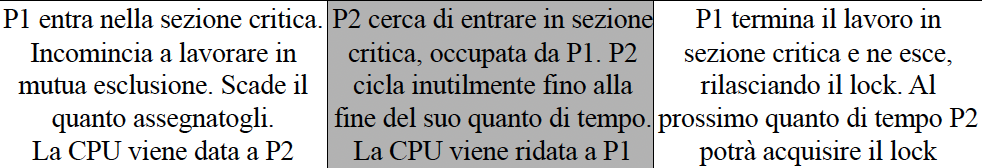
\includegraphics[width=0.5\linewidth]{images/busyWaiting_critics.png}
    \caption{Busy-Waiting}
    \label{fig:busyWaiting_critics}
\end{figure}
\clm{}{}{
E se invece di due processi ce ne sono $N$ che competono per acquisire lo stesso lock, un algoritmo di scheduling round robin potrebbe produrre uno spreco del tempo di CPU pari a $N-1$ quanti di temp.}

\section{Semafori}
\dfn{Semaforo}{
Strumento di sincronizzazione che, con l'aiuto del sistema operativo, può essere implementato senza \textit{busy-waiting}.}
\textbf{Definizione di Semaforo S:}
\begin{itemize}
    \item È una variabile intera (per ora assumiamo che sia inizializzata a 1) su cui si può operare solo tramite due operazioni atomiche (che descriviamo così, anche se non implementate in questo modo):
    \begin{itemize}
        \item \texttt{wait(S)}: 
        \begin{lstlisting}[language=C]
        while (S <= 0) do no-op;
        S = S - 1;
        \end{lstlisting}
        \item \texttt{signal(S)}: 
        \begin{lstlisting}[language=C]
        S = S + 1;
        \end{lstlisting}
    \end{itemize}
\end{itemize}
Un semaforo può essere visto come un \textbf{oggetto} condiviso da tutti i processi che devono usarlo per sincronizzarsi fra loro.
\begin{itemize}
    \item La variabile intera $S$ viene di solito chiamata \textit{variabile semaforica}, e il suo valore corrente è detto \textit{valore del semaforo}.
    \item \texttt{Wait} e \texttt{Signal} sono i metodi con cui si utilizza l'oggetto semaforo (in realtà, è necessaria anche un'operazione per inizializzare il valore della variabile semaforica).
\end{itemize}
In letteratura, i termini \texttt{Wait} e \texttt{Signal} sono talvolta sostituiti da termini olandesi, usati originariamente da Dijkstra:
\begin{itemize}
    \item \texttt{P} (\textit{Proberen} = verificare) al posto di \texttt{Wait};
    \item \texttt{V} (\textit{Verhogen} = incrementare) al posto di \texttt{Signal}.
\end{itemize}
Altri termini usati:
\begin{itemize}
    \item \texttt{Down} (per la \texttt{Wait}, che decrementa il semaforo);
    \item \texttt{Up} (per la \texttt{Signal}, che incrementa il semaforo).
\end{itemize}

\subsection{Uso dei semafori}
Adesso la soluzione del problema della sezione critica per un gruppo di processi è semplice. La variabile semaforica \texttt{mutex} (mutual exclusion) fa da variabile di \textit{lock}:

\begin{lstlisting}[language=C]
shared variable semaphore mutex = 1;

Generico processo Pi:
do {
    wait(mutex);
    // sezione critica
    signal(mutex);
    // sezione non critica
} while (true);
\end{lstlisting}
In realtà, i semafori possono essere usati per \textbf{qualsiasi} problema di \textbf{sincronizzazione} (ne vedremo più avanti alcuni relativamente complessi). 
Ad esempio, se vogliamo eseguire una generica operazione $S_1$ fatta dal processo $P_1$ prima di $S_2$, fatta dal processo $P_2$, possiamo usare un semaforo \texttt{sync} inizializzato a 0:
\begin{itemize}
    \item $P_1$ esegue:
    \begin{lstlisting}[language=C]
    S1;
    signal(sync);
    \end{lstlisting}
    \item $P_2$ esegue:
    \begin{lstlisting}[language=C]
    wait(sync);
    S2;
    \end{lstlisting}
\end{itemize}
\clm{}{}{
\textbf{Attenzione:} il nome scelto per un semaforo non ha nessuna relazione con l'uso che ne verrà fatto.}
\begin{itemize}
    \item Un semaforo è una \textbf{variabile} (in realtà, come vedremo tra poco, è una struttura dati) che ovviamente possiamo chiamare come preferiamo.
    \item Naturalmente, è meglio usare nomi che ricordino \textbf{l'uso che faremo} di un semaforo. Quindi, chiameremo \texttt{mutex} un semaforo usato per implementare una mutua esclusione, e \texttt{sync} un semaforo usato per implementare un meccanismo di sincronizzazione tra due processi.
    \item Ma non cambierebbe nulla se chiamassimo i due semafori rispettivamente \texttt{X} e \texttt{Y}, o anche \texttt{Pippo} e \texttt{Pluto}.
    \item Ciò che importa è \textbf{come li usiamo}.
\end{itemize}

\subsection{Implementazione dei semafori}
La definizione di \texttt{wait} e \texttt{signal} che abbiamo dato utilizza il \textit{busy-waiting}, e questo è proprio ciò che vorremmo evitare.

\begin{itemize}
    \item I semafori implementati attraverso il \textit{busy-waiting} esistono e prendono di solito il nome di \textit{spinlock} (nel senso che il processo "gira" mentre testa la variabile di lock, proprio come nelle tecniche di sincronizzazione via hardware).
    \item Per evitare il \textit{busy-waiting} dobbiamo farci aiutare dal Sistema Operativo, che mette a disposizione opportune strutture dati e \textit{system call} per l'implementazione delle operazioni di \texttt{wait} e \texttt{signal}.
\end{itemize}
Quando un gruppo di processi ha bisogno di un semaforo, lo richiede al Sistema Operativo tramite una \textit{system call}. 
\begin{itemize}
    \item Il SO alloca un nuovo semaforo all'interno di una lista di semafori memorizzata nelle aree dati del kernel.
    \item Ogni semaforo è implementato usando due campi: \texttt{valore} e \texttt{lista di attesa}.
\end{itemize}

\begin{lstlisting}[language=C]
typedef struct {
    int valore;
    struct processo *waiting_list;
} semaforo;
\end{lstlisting}
Due \textit{system call} sono disponibili per \textbf{implementare} le operazioni di \texttt{wait} e \texttt{signal}:
\begin{itemize}
    \item \texttt{sleep()}: toglie la CPU al processo che la invoca e manda in esecuzione uno dei processi nella Ready Queue. Il processo che ha chiamato \texttt{sleep} non viene rimesso nella Ready Queue (N.B.: a volte \texttt{sleep()} è chiamata \texttt{block()}).
    \item \texttt{wakeup(P)}: inserisce il processo $P$ nella Ready Queue.
\end{itemize}
Implementazione della \texttt{wait}:
\begin{lstlisting}[language=C]
wait(semaforo *S) {
    S->valore--;
    if (S->valore < 0) {
        aggiungi questo processo a S->waiting_list;
        sleep();
    }
}
\end{lstlisting}
La chiamata di \texttt{sleep()} provoca un \textit{context switch}, e il processo sospeso non consuma CPU inutilmente, poiché il suo PCB non è più nella Ready Queue, ma nella lista di attesa del semaforo su cui si è sospeso.
Si dice anche che il processo si è "\textbf{addormentato}" sul semaforo $S$.
\texttt{signal(semaforo *S)}:
\begin{lstlisting}[language=C]
signal(semaforo *S) {
    S->valore++;
    if (S->valore <= 0) { /* qualcuno in attesa */
        togli un processo P da S->waiting_list;
        wakeup(P);
    }
}
\end{lstlisting}

\textbf{Nota:} \texttt{wakeup(P)} rimette $P$ nella Ready Queue, quindi $P$ è pronto a usare la CPU quando sarà il suo turno. Si dice che $P$ è stato "svegliato".

\textbf{NOTATE BENE:} \texttt{wait} e \texttt{signal} sono di solito \textit{system call} direttamente messe a disposizione dal Sistema Operativo, anche se a volte con nomi diversi.
\begin{itemize}
    \item \texttt{wait} e \texttt{signal} sono esse stesse sezioni critiche. Perché? \textbf{(Perchè condividono delle variabili)}
    \item Sono sezioni critiche molto corte (circa 10 istruzioni macchina), quindi vanno bene implementate con \textit{spinlock} o disabilitazione degli interrupt (che avviene sotto il controllo del SO).
\end{itemize}

\qs{}{Quale soluzione è migliore per i sistemi monoprocessore e quale per i sistemi multiprocessore?}

\textbf{NOTATE ANCHE:} All'inizio, la semantica di \texttt{wait} era:
\begin{lstlisting}[language=C]
wait (S): 
    while (S <= 0) do no-op;
    S = S - 1;
\end{lstlisting}
\qs{}{Ma nell'implementazione tramite \texttt{sleep}, vediamo che il valore del semaforo può essere negativo. Come mai?}
\nt{Per conoscere quanti processi in un certo istante sono addormentanti}
\begin{itemize}
    \item Se $S->valore < 0$, il suo valore assoluto ci dice quanti processi sono in attesa (\textit{in wait}) su quel semaforo (si veda il codice della \texttt{wait}).
\end{itemize}
\textbf{NOTATE ANCORA:} Il valore del semaforo può anche essere un intero maggiore di 1. Ad esempio, se una risorsa può essere usata contemporaneamente da un massimo di tre processi:
\begin{lstlisting}[language=C]
semaphore counter = 3; // counter viene inizializzato a 3
Generico processo Pi:
repeat {
    wait(counter);
    // usa la risorsa
    signal(counter);
    // remainder section
} until false;
\end{lstlisting}        
\subsection{Riassunto}
Riassumendo, attraverso i semafori implementati usando \texttt{sleep()} e \texttt{wakeup(P)}, i processi utente possono contenere sezioni critiche arbitrariamente lunghe senza:
\begin{itemize}
    \item Sprecare inutilmente tempo di CPU (come accadrebbe se implementassimo le sezioni critiche con il \textit{busy-waiting}),
    \item Rischiare di dare il controllo della CPU al processo (come accadrebbe se si usasse la disabilitazione degli interrupt gestita direttamente dai processi utente).
\end{itemize}

\clm{}{}{
Le operazioni di \texttt{wait} e \texttt{signal} (che sono esse stesse sezioni critiche) possono invece essere implementate con \textit{busy-waiting} o disabilitazione degli interrupt, poiché queste operazioni durano poco tempo e avvengono sotto il controllo del Sistema Operativo.}


\section{Definizione di DeadLock}
\dfn{}{Si definisce \textbf{deadlock} di un sottoinsieme di processi del sistema \( \{P_1, P_2, \dots, P_n\} \subseteq P \) la situazione in cui ciascuno degli \( n \) processi \( P_i \) è in attesa del rilascio di una risorsa detenuta da uno degli altri processi del sottoinsieme;} si forma cioè una catena circolare per cui:

\[
P_1 \text{ aspetta } P_2 \dots \text{ aspetta } P_n \text{ aspetta } P_1
\]
Anche se non tutti i processi del sistema sono bloccati, la situazione non è desiderabile in quanto può bloccare alcune risorse e, di conseguenza, danneggiare anche i processi non coinvolti nel deadlock.




\section{Definizione di Starvation}
\dfn{}{Un processo è in \textbf{starvation} se non riesce mai a portare avanti la propria computazione.} Questo può accadere per diverse ragioni:

\begin{itemize}
    \item Non viene mai selezionato dallo \textit{scheduler} per entrare in esecuzione.
    \item Non riesce mai ad entrare in una sezione critica.
    \item Non riesce mai a prelevare una risorsa necessaria per proseguire la sua computazione.
\end{itemize}

\textbf{Nota:} Il \textit{deadlock} implica \textit{starvation}, ma non vale il contrario.

\section{Deadlock \& Starvation: (stallo e attesa indefinita)}
I \textbf{semafori} sono le primitive di sincronizzazione più semplici e più usate nei moderni Sistemi Operativi, e permettono di risolvere qualsiasi problema di sincronizzazione fra processi.

\begin{itemize}
    \item Tuttavia, sono primitive di sincronizzazione \textit{non strutturate} e quindi possono essere "rischiosi".
    \item Usando i semafori, non è difficile scrivere programmi che funzionano male, portando a situazioni di \textit{deadlock} o \textit{starvation}.
\end{itemize}

\textbf{Esempio}:
\begin{verbatim}
P_0          P_1
wait(S);     wait(Q);
wait(Q);     wait(S);
...          ...
signal(S);   signal(Q);
signal(Q);   signal(S);
\end{verbatim}

\qs{}{Se \( S \) e \( Q \) sono inizializzati a 1, cosa succede se \( P_0 \) e \( P_1 \) vengono eseguiti concorrentemente?}
\begin{itemize}
    \item Se dopo la \texttt{wait(S)} di \( P_0 \), la CPU viene assegnata a \( P_1 \), che esegue \texttt{wait(Q)}, e successivamente la CPU torna a \( P_0 \), \( P_0 \) non può più proseguire, causando così un \textbf{deadlock}.
\end{itemize}

\textbf{Problema dei semafori}: le operazioni \texttt{wait} e \texttt{signal} sono indipendenti e possono essere usate in modo errato. Esistono primitive di sincronizzazione più strutturate (es. \textit{Regioni Critiche Condizionali}, \textit{Monitor}) che possono evitare questi problemi.

\textbf{Approfondimento}: potete leggere la sezione 6.7 del testo per una descrizione del concetto di \textit{Monitor}.